\documentclass[12pt]{article}

\usepackage[utf8]{inputenc}
\usepackage[T1]{fontenc}
\usepackage{amsmath}
\usepackage{amssymb}
\usepackage{graphicx}
\usepackage{booktabs}
\usepackage{hyperref}
\usepackage[round]{natbib}
\usepackage{tikz}
\usetikzlibrary{positioning, arrows.meta, decorations.pathmorphing, calc, shapes.geometric}
\usepackage[margin=1in]{geometry}

\title{Sediment: How Streak Mechanics Drive Compelled Production of Low-Quality Digital Content}
\author{Jiyeon Yoon\\
Independent Researcher\\
\texttt{heznpc@gmail.com}}
\date{}

\begin{document}

\maketitle

\begin{abstract}
Streak mechanics---design features that reward consecutive-day activity with visible counters, badges, or social obligations---are among the most widely deployed motivational tools in consumer software. Duolingo, GitHub, Snapchat, and hundreds of fitness, writing, and productivity applications rely on streaks to sustain daily engagement. Yet the same mechanic that encourages consistent practice also compels users to produce low-quality filler content on days when they have nothing meaningful to contribute, simply to avoid losing an accumulated record. We introduce the concept of \emph{sediment}: digital content whose informational value falls below a platform-contextual quality threshold, defined by its properties rather than its cause. Drawing on a geological metaphor, we propose a three-stage lifecycle model---Deposition, Compaction, and Fossilization---each generating distinct, testable predictions about how filler content accumulates, degrades platform signal-to-noise ratios, and acquires unwarranted social legitimacy over time. We develop three competing psychological hypotheses (loss aversion under temporal visibility, identity-consistency pressure, and escalating commitment) and propose four studies to test them: (1) a GitHub observational analysis with a natural experiment exploiting the 2016 streak counter removal, (2) a controlled $2 \times 2$ streak UI experiment, (3) a cross-platform survey with embedded mechanism discrimination, and (4) a fossilization vignette study examining how streak-pattern contribution graphs bias developer evaluations. We further theorize that AI code-generation tools such as GitHub Copilot amplify streak-driven filler by collapsing the effort cost that would otherwise break the streak. We conclude with design implications for quality-preserving streak alternatives, including rolling windows, quality-gated streaks, and post-habit-window transitions.
\end{abstract}

% ============================================================
% SECTION 1: INTRODUCTION
% ============================================================
\section{Introduction}
\label{sec:introduction}

\subsection{The Streak Paradox}
\label{sec:streak-paradox}

On any given day, thousands of software developers push trivial commits---a whitespace change, a one-line README edit, an empty configuration file---to their GitHub repositories. They do so not because the code needs changing, but because their contribution graph demands a green square. In Korean developer communities, the practice has its own name: \emph{1il 1keomis} (``one day, one commit''), a daily discipline that began as a self-improvement ethos and hardened into an obligation enforced by social expectation and visual design. The developers producing these commits frequently know the output is meaningless. They push the code anyway.

This behavior is not confined to software development. Duolingo learners complete perfunctory lessons---tapping through the easiest available exercise without reading the prompts---to preserve streaks that may span hundreds of days. Snapchat users exchange blank images or single-character messages to maintain ``Snapstreaks'' with friends, sustaining a counter that resets to zero if either party fails to send a snap within 24 hours. Fitness application users log fabricated workouts. Writers on daily-blogging platforms publish placeholder posts. In each case, the pattern is the same: a platform mechanic designed to encourage consistent engagement instead compels the production of content that nobody---not the producer, not any consumer, not the platform itself---actually wants.

The content produced through these rituals is not ephemeral. It persists on platform timelines indefinitely: in commit histories that future collaborators must parse, in language-learning progress records that misrepresent actual proficiency, in social media feeds that bury meaningful posts beneath a layer of filler. This accumulated residue constitutes a previously unexamined category of low-quality digital content---one that is human-generated, platform-compelled, and demand-independent. Unlike spam, it is produced by legitimate users acting in good faith within the incentive structures they have been given. Unlike AI-generated ``slop,'' it is not the product of cheap supply but of artificially manufactured demand. We propose the term \emph{sediment} for this category and develop a theoretical framework for understanding its production, accumulation, and consequences.

\subsection{Compelled Production}
\label{sec:compelled-production}

Recent scholarship on digital content quality has focused predominantly on the supply side: generative AI makes content production cheap, flooding platforms with machine-generated text, images, and code of uncertain quality. This supply-side framing captures an important dynamic but overlooks a complementary mechanism that operates on the demand side. Streak mechanics do not merely make production easy; they make production \emph{obligatory}. The user interface imposes a production quota---one unit per day, every day, regardless of whether the user has anything worth producing---and enforces it through the threat of visible loss.

The critical distinction is that compelled production is demand-independent. In conventional economic models of content production, supply responds to demand: creators produce because audiences consume, advertisers pay, or intrinsic satisfaction rewards the effort. Streak-driven filler violates this model. Nobody requests the whitespace commit. No audience awaits the blank Snapchat image. No learning outcome depends on the perfunctory Duolingo lesson. The production quota exists because the user interface creates it, not because any downstream consumer benefits from its fulfillment.

When AI tools are available, this quota becomes trivially satisfiable. A developer maintaining a GitHub streak can prompt Copilot to generate a plausible commit in seconds. A blogger can ask ChatGPT to produce a passable daily post. The effort cost that might otherwise have broken the streak---forcing the user to either produce something genuine or accept the loss---collapses to near zero. AI thus functions not as a content creation tool in the conventional sense, but as a streak maintenance tool: a technology whose primary value, in this context, is preserving a counter that the user would prefer not to lose.

\subsection{Streaks Work---And That's Precisely the Question}
\label{sec:streaks-work}

An important caveat must precede any critique of streak mechanics: they work. Duolingo's internal data consistently identifies streaks as the company's single most effective retention feature. Users with active streaks return to the application at dramatically higher rates than users without them. Controlled experiments in health behavior have demonstrated that loss-framed incentives, which share the psychological structure of streak mechanics, significantly increase physical activity relative to gain-framed alternatives \citep{Patel2016}. The broader gamification literature, while subject to publication bias and methodological concerns \citep{Koivisto2019}, reports generally positive effects of progress-tracking features on motivation and engagement \citep{Hamari2014, Sailer2017}.

The habit formation literature provides a theoretical basis for these effects. \citet{Lally2010} found that new behaviors require an average of 66 days of consistent repetition to reach automaticity, with substantial individual variation around this mean. Streak mechanics directly support this formation window by providing external scaffolding---a visible record of consistency and a penalty for interruption---during the period when the new behavior has not yet become self-sustaining.

The question this paper investigates is therefore not whether streaks are beneficial in the abstract, but \emph{when and how} their benefits degrade into compelled filler production. Current streak designs are indiscriminate: they reward any output on any day with equal credit, treating a substantive code contribution and a whitespace edit as interchangeable so long as both register on the contribution graph. This indiscriminacy is a design choice, not a necessity. It is possible in principle to design streak mechanics that reward quality, that tolerate planned rest days, or that transition from consistency tracking to quality tracking after the habit formation window has closed. That such designs are rare in practice suggests that the indiscriminate version serves platform engagement metrics even as it generates negative externalities for content ecosystems. We propose a boundary condition hypothesis: streak mechanics primarily support genuine engagement within the approximately 66-day habit formation window identified by \citet{Lally2010}; beyond this window, they increasingly produce diminishing motivational returns and escalating filler.

\subsection{Research Questions}
\label{sec:research-questions}

\begin{description}
    \item[RQ1:] Do streak mechanics increase the proportion of low-quality content production, and does this effect intensify with streak length?
    \item[RQ2:] What psychological mechanisms mediate the relationship between streak mechanics and content quality degradation? Specifically: does loss aversion under temporal visibility, identity-consistency pressure, or escalating commitment best explain the effect?
    \item[RQ3:] Does AI tool availability moderate (amplify) streak-driven filler production by removing the effort cost that would otherwise break the streak?
\end{description}

% ============================================================
% SECTION 2: THEORETICAL FRAMEWORK
% ============================================================
\section{Theoretical Framework}
\label{sec:theoretical-framework}

\subsection{Sediment: Definition and Model}
\label{sec:sediment-definition}

\subsubsection{Definition}
\label{sec:definition}

\textbf{Sediment} is defined as digital content whose informational value falls below a platform-contextual quality threshold, measured independently of its production context. Sediment is defined by its properties---low signal, persistence, accumulation---not by its cause.

This cause-independent definition is methodologically essential. If we were to define sediment as ``content produced to maintain a streak,'' any finding that streaks produce sediment would be circular. Instead, we first establish what sediment \emph{is}---content that falls below a quality threshold calibrated to the norms and expectations of a given platform context---and then empirically test whether streak mechanics produce more of it. A whitespace-only commit qualifies as sediment on GitHub not because it was produced to maintain a streak, but because it adds no informational value to the repository. That the same commit may also have been produced under streak pressure is an empirical finding, not a definitional entailment.

The platform-contextual quality threshold acknowledges that content quality is not absolute. A brief personal update may be perfectly appropriate on a social media feed but would constitute sediment if pushed as a commit to a professional software repository. Operationalizing this threshold requires domain-specific calibration, which we address through the ground truth validation in Study~1a.

\subsubsection{The Sediment Model}
\label{sec:sediment-model}

The term \emph{sediment} invokes a geological metaphor that captures the essential dynamics of streak-driven filler accumulation more precisely than alternative framings such as ``noise,'' ``clutter,'' or ``pollution.'' In fluvial geomorphology, sediment consists of fine particles carried by water flow that are individually invisible but collectively reshape the landscape over time. No single particle of silt is consequential; it is the cumulative deposit that reshapes the riverbed, buries prior formations, and alters the course of future flow.

Platform timelines operate analogously. Each individual filler commit, perfunctory lesson completion, or placeholder post is trivial in isolation. But accumulated across thousands of users and hundreds of days, these deposits reshape the informational landscape: commit histories become harder to navigate, search results return lower-quality matches, and contribution graphs encode misleading signals about developer activity. The metaphor captures three properties that distinguish sediment from other forms of low-quality content. First, \emph{passivity}: unlike erosion, which actively destroys existing content, sedimentation passively accumulates alongside it, gradually reducing the signal-to-noise ratio without deleting anything. Second, \emph{persistence}: sediment, once deposited, tends to remain indefinitely, as platforms rarely provide mechanisms or incentives for its removal. Third, \emph{invisibility at the individual level}: no single piece of filler triggers alarm, but the cumulative deposit fundamentally degrades the information environment.

The sediment framework is, at its core, an application of Goodhart's Law to temporal consistency metrics in gamified platforms. \citet{Goodhart1975} observed that when a measure becomes a target, it ceases to be a good measure; \citet{Strathern1997} generalized this principle to audit cultures more broadly. Streak counters are a textbook instantiation: platform designers adopt daily activity frequency as a proxy for genuine engagement, then make that proxy visible to users as a target to pursue. Once users optimize for frequency rather than quality, the proxy decouples from the underlying construct it was meant to measure, and the resulting metric inflation produces the very sediment we seek to study.

\subsubsection{Sediment Lifecycle: Deposition, Compaction, Fossilization}
\label{sec:lifecycle}

We propose that sediment follows a three-stage lifecycle, each characterized by a distinct mechanism and generating distinct, testable predictions.

\begin{figure}[htbp]
\centering
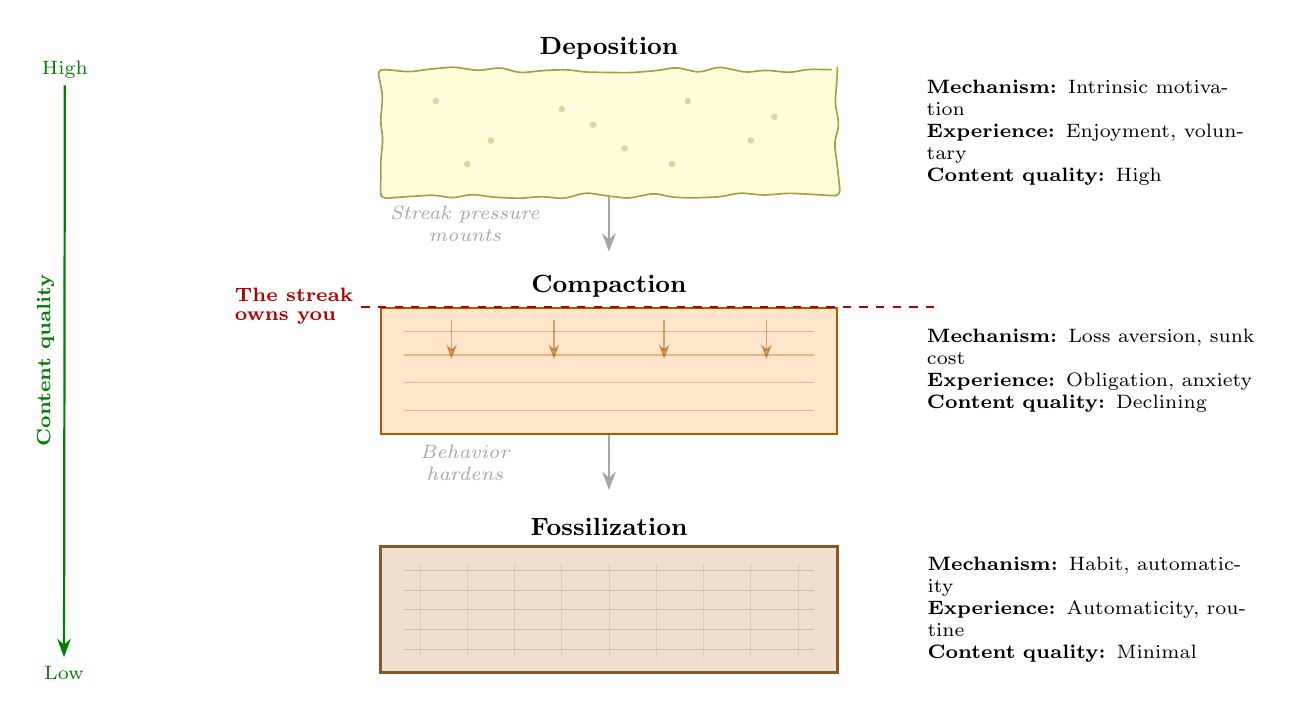
\begin{tikzpicture}[
    >=Stealth,
    layer/.style={
        minimum width=5.8cm,
        minimum height=1.6cm,
        text width=5.4cm,
        align=center,
        font=\small,
    },
    annot/.style={
        font=\scriptsize,
        text width=4.2cm,
        align=left,
    },
    stage label/.style={
        font=\bfseries\small,
    },
    arrow label/.style={
        font=\scriptsize\itshape,
        text width=2.8cm,
        align=center,
    },
]

% --- Stage 1: Deposition (top, loose sediment) ---
\node[layer,
    fill=yellow!15,
    draw=yellow!60!black,
    line width=0.6pt,
    rounded corners=2pt,
    decorate, decoration={random steps, segment length=8pt, amplitude=1.2pt},
] (dep) {};

\node[stage label, above=0pt of dep.north] {Deposition};

\node[annot, right=1.0cm of dep.east, anchor=west] (dep-annot) {%
    \textbf{Mechanism:} Intrinsic motivation\\
    \textbf{Experience:} Enjoyment, voluntary\\
    \textbf{Content quality:} High%
};

% Scattered dots to suggest loose particles
\foreach \x/\y in {-2.2/0.4, -1.5/-0.1, -0.6/0.3, 0.2/-0.2, 1.0/0.4, 1.8/-0.1, -0.2/0.1, 0.8/-0.4, -1.8/-0.4, 2.1/0.2} {
    \fill[yellow!60!black, opacity=0.4] ([shift={(\x cm, \y cm)}]dep.center) circle (1.2pt);
}

% --- Transition arrow 1 ---
\draw[->, thick, gray!70] (dep.south) -- ++(0, -0.7)
    node[arrow label, midway, left=0.3cm] {Streak pressure\\mounts};

% --- Stage 2: Compaction (middle, compressed layers) ---
\node[layer,
    fill=orange!20,
    draw=orange!70!black,
    line width=0.8pt,
    below=1.4cm of dep,
] (comp) {};

\node[stage label, above=0pt of comp.north] {Compaction};

\node[annot, right=1.0cm of comp.east, anchor=west] (comp-annot) {%
    \textbf{Mechanism:} Loss aversion, sunk cost\\
    \textbf{Experience:} Obligation, anxiety\\
    \textbf{Content quality:} Declining%
};

% Horizontal compression lines
\foreach \y in {-0.5, -0.15, 0.2, 0.5} {
    \draw[orange!70!black, opacity=0.35, line width=0.4pt]
        ([shift={(-2.6cm, \y cm)}]comp.center) -- ([shift={(2.6cm, \y cm)}]comp.center);
}

% --- Ownership inversion marker ---
\draw[red!70!black, thick, dashed] ([shift={(-4.2cm, 0)}]comp.north) -- ([shift={(4.2cm, 0)}]comp.north);
\node[font=\scriptsize\bfseries, text=red!70!black, fill=white, inner sep=2pt]
    at ([shift={(-4.0cm, 0)}]comp.north) {%
    \begin{tabular}{@{}l@{}}
        The streak\\[-1pt] owns you
    \end{tabular}%
};

% Downward pressure arrows
\foreach \x in {-2.0, -0.7, 0.7, 2.0} {
    \draw[->, orange!70!black, opacity=0.5, line width=0.5pt]
        ([shift={(\x cm, 0.65cm)}]comp.center) -- ([shift={(\x cm, 0.15cm)}]comp.center);
}

% --- Transition arrow 2 ---
\draw[->, thick, gray!70] (comp.south) -- ++(0, -0.7)
    node[arrow label, midway, left=0.3cm] {Behavior\\hardens};

% --- Stage 3: Fossilization (bottom, solid rock) ---
\node[layer,
    fill=brown!25,
    draw=brown!70!black,
    line width=1.2pt,
    below=1.4cm of comp,
] (foss) {};

\node[stage label, above=0pt of foss.north] {Fossilization};

\node[annot, right=1.0cm of foss.east, anchor=west] (foss-annot) {%
    \textbf{Mechanism:} Habit, automaticity\\
    \textbf{Experience:} Automaticity, routine\\
    \textbf{Content quality:} Minimal%
};

% Dense cross-hatching for rock texture
\foreach \y in {-0.5, -0.25, 0.0, 0.25, 0.5} {
    \draw[brown!70!black, opacity=0.25, line width=0.3pt]
        ([shift={(-2.6cm, \y cm)}]foss.center) -- ([shift={(2.6cm, \y cm)}]foss.center);
}
\foreach \x in {-2.4, -1.8, -1.2, -0.6, 0.0, 0.6, 1.2, 1.8, 2.4} {
    \draw[brown!70!black, opacity=0.15, line width=0.3pt]
        ([shift={(\x cm, -0.6cm)}]foss.center) -- ([shift={(\x cm, 0.6cm)}]foss.center);
}

% --- Content quality trajectory arrow (left side) ---
\draw[->, thick, green!50!black]
    ([shift={(-4.0cm, 0.6cm)}]dep.west) -- ([shift={(-4.0cm, -0.6cm)}]foss.west)
    node[midway, rotate=90, above=4pt, font=\scriptsize\bfseries] {Content quality};
\node[font=\scriptsize, green!50!black] at ([shift={(-4.0cm, 0.8cm)}]dep.west) {High};
\node[font=\scriptsize, green!50!black] at ([shift={(-4.0cm, -0.8cm)}]foss.west) {Low};

\end{tikzpicture}
\caption{The Sediment Lifecycle Model. Content produced under streak mechanics progresses through three geological stages. During \emph{Deposition}, engagement is voluntary and content quality is high. As streak pressure intensifies, \emph{Compaction} sets in: loss aversion and sunk-cost reasoning transform participation from choice into obligation---the point at which ``the streak owns you'' rather than ``you own the streak'' (dashed line). In \emph{Fossilization}, the behavior persists as automaticity even as content quality reaches its minimum, and the accumulated record acquires unwarranted social legitimacy as a credentialing signal.}
\label{fig:lifecycle}
\end{figure}

\paragraph{Deposition.}
The first stage is the act of filler production itself. Under streak pressure, users create content whose primary purpose is to fill a temporal gap in their activity record. The producer is frequently aware that the content is low-quality---developers describe their streak-maintenance commits as ``garbage,'' ``throwaway,'' or ``just keeping the streak alive''---but produces it anyway because the perceived cost of breaking the streak exceeds the perceived cost of depositing filler. Deposition is thus a conscious, if reluctant, response to a platform-imposed production quota.

This stage generates a directly testable prediction: the proportion of below-threshold content should increase on \emph{streak-risk days}---days on which a user's streak would break if no activity is recorded---relative to non-streak-risk days for the same user. Study~1b is designed to test this prediction by comparing content quality metrics on streak-risk days versus non-risk days within individual users' contribution histories.

\paragraph{Compaction.}
The second stage describes the cumulative effect of sustained deposition on the information environment. As filler accumulates, it compresses the signal in a repository, feed, or search index. Repositories with high filler ratios become harder to navigate: meaningful commits are buried among trivial edits, code review becomes more effortful, and new contributors face a noisier onboarding experience. At the platform level, search and recommendation algorithms trained on sediment-laden data may amplify low-quality content, further degrading discoverability.

The compaction stage generates a longitudinal prediction: repositories that accumulate higher proportions of filler over time should exhibit declining engagement metrics---fewer stars, fewer forks, fewer new contributors, and slower issue response times---compared to repositories with similar activity levels but lower filler ratios. Study~1d tests this prediction using rolling signal-to-noise ratios computed over repositories with two or more years of history.

\paragraph{Fossilization.}
The third stage occurs when accumulated sediment acquires social legitimacy. A 365-day contribution graph on GitHub, regardless of the quality of the underlying commits, is widely interpreted as a signal of diligence, discipline, and technical commitment. Hiring managers and technical recruiters routinely consult contribution graphs when evaluating developer candidates, treating streak patterns as evidence of competence. The sediment has \emph{fossilized}: it has hardened from disposable filler into a durable social credential that influences real-world decisions.

Fossilization generates a prediction testable through vignette experiments: evaluators should rate developer profiles with streak-pattern contribution graphs more favorably than equivalent profiles with sporadic contribution patterns, even when the underlying code quality is identical or lower. Study~4 is designed to test this prediction and to assess whether the fossilization bias is stronger among evaluators who use GitHub profiles in actual hiring decisions.

\subsection{Psychological Mechanisms (Competing Hypotheses)}
\label{sec:psychological-mechanisms}

We propose three competing psychological mechanisms that may explain why users continue to produce filler under streak pressure. These hypotheses are not mutually exclusive---multiple mechanisms may operate simultaneously---but they generate distinguishable predictions that allow empirical discrimination.

\subsubsection{H1: Loss Aversion Under Temporal Visibility}
\label{sec:h1-loss-aversion}

Prospect theory \citep{Kahneman1979} predicts that losses are weighted more heavily than equivalent gains. Streak mechanics transform a neutral absence---a day without activity---into a visible loss: a gap in a contribution graph, a counter reset to zero, a broken fire icon. The key feature of this mechanism is \emph{temporal visibility}: the loss is not merely experienced internally but displayed on a timeline that is visible to both the user and others. This social proof dimension connects streak anxiety to the broader literature on fear of missing out (FOMO; \citealp{Yu2025}) and the intolerance of visible incompleteness.

H1 predicts that filler production is primarily driven by the visual display of streaks, not by streak length per se. If loss aversion under temporal visibility is the dominant mechanism, then filler should increase whenever streaks are visually salient---regardless of whether the streak is 5 days or 500 days long---and should decrease when the visual display is removed or hidden.

\subsubsection{H2: Identity-Consistency Pressure}
\label{sec:h2-identity}

The second hypothesis draws on the consistency principle \citep{Cialdini1984}, cognitive dissonance theory \citep{Festinger1957}, and identity-based motivation \citep{Oyserman2007}. Users who maintain long streaks may internalize the streak as part of their self-concept: ``I am a person who commits every day,'' ``I am a 500-day Duolingo learner.'' A gap in the streak does not merely register as a loss; it threatens the identity narrative. Producing filler becomes an act of identity maintenance rather than a rational response to a sunk cost.

From the perspective of self-determination theory \citep{Ryan2000}, this mechanism reveals a tension within streak mechanics: streaks may satisfy the need for competence (by providing tangible evidence of consistency and progress) while simultaneously eroding autonomy (by constraining the user's freedom to take a day off without psychological cost). When competence satisfaction depends on continued streak maintenance, the user faces a choice between autonomy and competence that filler resolves in favor of the latter.

H2 predicts that filler production is driven by the centrality of the streak to the user's self-concept, independent of streak length. Users who strongly identify with their streak (``This streak is part of who I am'') should produce more filler than users who view their streak instrumentally (``The streak helps me practice''), regardless of whether their streak is short or long.

\subsubsection{H3: Escalating Commitment}
\label{sec:h3-escalating-commitment}

The third hypothesis invokes the escalation of commitment to a failing course of action \citep{Staw1976}. Streak counters manufacture the perception of sunk investment where none objectively exists: a 200-day streak has no material value---no transferable asset, no redeemable reward---yet users describe ``losing'' a long streak in terms that suggest genuine financial or emotional loss. This manufactured sunk cost triggers the same escalation dynamics observed in organizational decision-making, where decision-makers continue investing in failing projects to justify prior investment \citep{Brockner1992}. The longer the streak, the greater the perceived sunk cost, and the more the user is willing to degrade content quality to avoid ``wasting'' the accumulated record.

The concept of entrapment is particularly apt: the user enters the streak voluntarily, finds each incremental day easy to justify, and discovers only gradually that the accumulated commitment has become a binding constraint on daily behavior. By the time the streak is long enough to feel costly to break, the user has already invested far more time in maintenance than the streak's objective value warrants.

H3 predicts that filler production increases monotonically with streak length, regardless of whether the streak is visually displayed or central to the user's identity. The key moderator is the magnitude of perceived accumulated investment, which is directly indexed by the streak counter.

\subsubsection{Distinguishing the Hypotheses}
\label{sec:distinguishing-hypotheses}

\begin{table}[ht]
\centering
\caption{Discriminating predictions for the three hypothesized mechanisms.}
\label{tab:hypotheses}
\begin{tabular}{llll}
\toprule
Mechanism & Key moderator & Filler driven by & Filler drops when \\
\midrule
H1: Loss aversion & Display salience & Gap visibility & Display is hidden \\
H2: Identity-consistency & Identity centrality & Self-concept threat & Low identification \\
H3: Escalating commitment & Streak length & Perceived investment & Streak is short \\
\bottomrule
\end{tabular}
\end{table}

Table~\ref{tab:hypotheses} summarizes the discriminating predictions. The three hypotheses converge in predicting that streak mechanics increase filler production, but they diverge on the conditions under which filler should increase or decrease. Study~3 is designed to discriminate between them by measuring all three proposed moderators (display salience, identity centrality, and streak length) simultaneously in a path model that allows their relative explanatory power to be compared. If H1 is dominant, display salience should be the strongest predictor of filler and should mediate the streak--filler relationship; if H2 is dominant, identity centrality should carry the mediation; if H3 is dominant, streak length should predict filler independently of the other two moderators. The natural experiment in Study~1c provides complementary evidence: the 2016 removal of GitHub's streak counter directly manipulated display salience (testing H1) while leaving streak length and identity centrality unchanged (holding H2 and H3 constant).

\subsection{Quality--Continuity Tradeoff}
\label{sec:quality-continuity}

Streak mechanics impose a daily production requirement regardless of available input---the user's ideas, energy, time, or material to work with on a given day. On high-input days, the streak requirement is costless: the user would have produced content anyway. On low-input days, however, the user faces a forced choice between breaking the streak and producing filler. This is the quality--continuity tradeoff: the streak mechanic demands temporal continuity at the potential expense of content quality.

Two competing sub-models describe how this tradeoff operates. Under the \emph{substitution model}, filler crowds out quality: on low-input days, the user's limited time and effort are allocated to producing a minimally viable streak-maintenance contribution rather than working on a more substantive task that might span multiple days. Under the \emph{additive model}, filler is produced on top of normal output---it represents additional, low-quality content that would not have been created in the absence of the streak mechanic, without displacing quality contributions. The distinction matters for assessing the net welfare effect of streaks. If the additive model holds, streaks impose costs (noise, false signals) but do not reduce the absolute quantity of quality content. If the substitution model holds, streaks not only add noise but actively reduce the production of quality content by fragmenting work into daily units.

Study~1b is designed to test between these models by examining whether total quality-weighted output decreases on streak-risk days (substitution) or remains constant while below-threshold output increases (additive). The controlled experiment in Study~2 provides a complementary test by comparing quality output across streak-visible and streak-hidden conditions. Evidence from the mandatory gamification literature suggests that the substitution model is more likely: \citet{Mollick2014} found that gamification harms performance outcomes when it is perceived as mandatory rather than voluntary, precisely the condition that streak mechanics impose.

\subsection{AI as Streak Maintenance Tool}
\label{sec:ai-streak-tool}

The emergence of AI code generation tools introduces a qualitatively new dynamic into the streak--filler relationship. Before AI assistants such as GitHub Copilot and ChatGPT became widely available, producing even low-quality streak-maintenance content required non-trivial effort: the developer had to open an editor, think of something to change, write the code, and push the commit. This effort cost served as a natural quality filter---a friction point that, at some threshold of inconvenience or fatigue, would cause the user to break the streak rather than produce filler. After AI, this filter is effectively removed. A developer can prompt Copilot to generate a plausible-looking function, accept the suggestion without review, and commit the result in under a minute. The effort cost of filler production collapses to near zero.

The specific interaction mechanism we propose is that AI reduces the \emph{decision threshold} for filler production. Without AI, a user on a low-input day faces a cost--benefit calculation: is the streak worth 20 minutes of producing something I know is trivial? With AI, the same calculation shifts: is the streak worth 30 seconds of accepting a generated suggestion? The expected answer changes, and the behavioral outcome shifts toward filler production. ChatGPT serves an analogous function for daily blog posts, daily journal entries, and other text-based streak obligations: it transforms the decision from ``Do I have something to write about today?'' into ``Should I ask the AI to write something for me today?''

This mechanism is measurable in observational data. Study~1b includes an AI moderation analysis that identifies Copilot-suggestive commit patterns---commits that exhibit characteristics consistent with AI generation, such as boilerplate function signatures, unusually uniform formatting, or commit messages that follow AI-typical templates---and tests whether the association between streak pressure and filler production is stronger for commits exhibiting these patterns. We hypothesize that the streak $\times$ AI interaction effect on filler production is positive and significant: AI availability amplifies the filler-producing effect of streak mechanics by removing the effort cost that would otherwise serve as a natural brake on sediment deposition.

\subsection{Who Bears the Cost?}
\label{sec:who-bears-cost}

\subsubsection{The Producer}
\label{sec:cost-producer}

The first and most immediate cost falls on the user who produces the filler. Streak-driven filler production erodes intrinsic motivation through the overjustification effect: as the extrinsic reward of streak maintenance becomes the dominant reason for engaging in an activity, the intrinsic interest that originally motivated participation declines \citep{Deci1999}. A developer who began committing daily to improve their craft gradually finds that the streak itself has become the purpose, and the craft improvement has become incidental.

This erosion often manifests as an anxiety--guilt cycle. The streak creates daily pressure to produce; on low-input days, the user responds with low-quality output; awareness of the low quality generates guilt or dissatisfaction; the dissatisfaction intensifies the pressure to ``make up for it'' on subsequent days, which paradoxically increases vulnerability to further filler production. \citet{Hanus2015} documented a related pattern in educational gamification, where students exposed to gamification elements reported lower intrinsic motivation and academic performance over a semester-long longitudinal study---precisely the kind of long-term degradation that streak mechanics may produce.

\subsubsection{The Consumer / Information Seeker}
\label{sec:cost-consumer}

The second cost falls on anyone who subsequently encounters the accumulated sediment. In software development, this includes future collaborators who must navigate commit histories laden with trivial changes, code reviewers whose attention is divided across meaningful and meaningless pull requests, and new contributors who encounter a noisy repository and struggle to identify relevant entry points.

A particularly consequential form of consumer cost is false credentialing. GitHub contribution graphs are widely used in hiring evaluations as a proxy for developer activity and commitment. When streak-maintained graphs misrepresent the quality of underlying contributions, hiring managers make decisions based on a corrupted signal. The fossilization stage of the sediment lifecycle makes this cost explicit: filler that was trivial at the time of production acquires durable social authority as it hardens into a visible record of apparent diligence. Trust erosion follows: as the gap between contribution graph signals and actual contribution quality becomes known, the credibility of the entire metric system degrades, harming both producers who maintain genuine streaks and consumers who rely on the signal.

\subsubsection{The Platform}
\label{sec:cost-platform}

The third cost falls on the platform itself, though it may not be recognized as such. Recommendation and search algorithms trained on sediment-laden data may learn to amplify low-quality content, creating a feedback loop in which filler begets visibility and visibility begets more filler. Moderation systems face a novel challenge: streak-driven filler is not spam (it is produced by legitimate users in compliance with platform norms), not abuse (it violates no policies), and not AI-generated slop in the conventional sense (it may be human-authored). It is, instead, a structural byproduct of the platform's own design choices---a category that existing content moderation taxonomies are ill-equipped to address.

\subsection{Hypotheses}
\label{sec:hypotheses}

The theoretical framework developed above generates the following testable hypotheses, organized by the three stages of the sediment lifecycle and the proposed moderating mechanisms. Each hypothesis specifies the predicted direction and is designed to be empirically falsifiable through the studies proposed in Section~\ref{sec:methodology}.

\paragraph{H1 (Deposition).} The proportion of below-threshold content (sediment) produced by a user is significantly higher on streak-risk days than on non-streak-risk days within the same user's contribution history. \textit{(Tested in Study~1b.)}

\paragraph{H2 (Compaction).} Repositories that accumulate a higher proportion of sediment over time exhibit significantly lower engagement metrics (stars, forks, new contributors, issue response speed) than repositories with comparable activity levels but lower sediment ratios. \textit{(Tested in Study~1d.)}

\paragraph{H3 (Fossilization).} Evaluators rate developer profiles with streak-pattern contribution graphs as significantly more competent than profiles with sporadic contribution patterns, even when the underlying code quality of the sporadic profile is equal to or higher than that of the streak profile. \textit{(Tested in Study~4.)}

\paragraph{H4 (Mechanism---Loss Aversion).} If loss aversion under temporal visibility is the dominant psychological driver of filler production, then removing or hiding the visual streak display will significantly reduce filler production, regardless of streak length or identity centrality. \textit{(Tested in Studies~1c and~2.)}

\paragraph{H5 (Mechanism---Identity-Consistency).} If identity-consistency pressure is the dominant driver, then self-concept centrality of the streak (``This streak is part of who I am'') will be a stronger predictor of filler production than either streak length or display salience. \textit{(Tested in Study~3b.)}

\paragraph{H6 (Mechanism---Escalating Commitment).} If escalating commitment is the dominant driver, then filler production will increase monotonically with streak length, regardless of whether the streak is visually displayed or central to the user's identity. \textit{(Tested in Studies~1c and~3b.)}

\paragraph{H7 (AI Amplification).} The interaction effect of streak pressure $\times$ AI tool availability on filler production is positive and significant: AI availability amplifies the filler-producing effect of streak mechanics by reducing the effort cost that would otherwise limit sediment deposition. \textit{(Tested in Studies~1b and~2.)}

\paragraph{H8 (Quality--Continuity Tradeoff).} Total quality-weighted output decreases on streak-risk days relative to non-risk days (substitution model), rather than remaining constant while below-threshold output increases (additive model). \textit{(Tested in Studies~1b and~2.)}

\paragraph{H9 (Boundary Condition).} The positive motivational effect of streak mechanics on content quality is concentrated within the approximately 66-day habit formation window; beyond this window, the proportion of sediment increases significantly while quality-weighted output shows diminishing returns. \textit{(Tested in Study~2.)}

% ============================================================
% SECTION 3: LITERATURE REVIEW
% ============================================================
\section{Literature Review}
\label{sec:literature-review}

\subsection{Persuasive Technology and Dark Patterns}
\label{sec:lit-persuasive-tech}

The sediment framework builds on the persuasive technology tradition established by \citet{Fogg2003}, whose Behavior Model (B = MAP) identifies motivation, ability, and prompts as the three necessary conditions for behavior change. Streak mechanics map cleanly onto this model: loss aversion provides the motivation; the platform interface provides the ability (by setting a low bar for what ``counts'' as daily activity); and the streak counter itself serves as a persistent, daily prompt. AI tools amplify the ability component by reducing the effort required to produce content that satisfies the prompt.

The dark patterns literature provides a complementary lens. \citet{Gray2018} developed a taxonomy of manipulative design patterns that includes ``forced action'' (requiring users to perform an action to access functionality) and ``nagging'' (persistent, repeated prompts). Streak mechanics exhibit features of both: they force daily action to preserve a valued record and nag through visual cues (dimmed squares, broken chains, declining counters). \citet{Mathur2019} demonstrated the prevalence of dark patterns at scale across commercial websites, establishing methodological precedents relevant to the large-scale observational analysis in Study~1. \citet{Brignull2010} described the ``roach motel'' pattern---easy to get into, hard to get out of---which aptly characterizes long streaks that users feel trapped by.

\citet{Eyal2014} offered a related framework in the Hooked model, which identifies four stages of habit-forming product design: trigger, action, variable reward, and investment. Streaks function as the investment phase: each day of streak maintenance increases the user's perceived investment, making it psychologically costlier to disengage. The sediment framework extends these perspectives by shifting attention from the moment of manipulation to its cumulative content externality. Dark patterns research has traditionally focused on the user's experience at the point of interaction; sediment theory examines what happens to the \emph{content} that manipulation produces after it is deposited on the platform.

\subsection{Operant Conditioning and Behavioral Compulsion}
\label{sec:lit-operant}

From a behaviorist perspective, streak mechanics implement a fixed-interval reinforcement schedule with a punishment contingency \citep{Skinner1953}. The user receives reinforcement (streak continuation) at fixed 24-hour intervals, contingent on producing at least one unit of output; failure to produce triggers punishment (streak reset). This schedule predicts characteristic behavioral patterns: escalation of effort as the deadline approaches (end-of-day streak-saving commits), resistance to extinction (continued streak maintenance long after the underlying behavior has ceased to serve its original purpose), and emotional distress at the prospect of schedule disruption.

\citet{Schull2012} identified structural parallels between addictive gambling machine design and other technologies that exploit fixed-interval reinforcement, noting that the ``zone'' of compulsive machine gambling shares phenomenological features with compulsive streak maintenance: reduced awareness of time, narrowed attention to the immediate reinforcement cycle, and continuation despite awareness that the behavior is no longer rewarding. \citet{Griffiths2005} proposed a components model of behavioral addiction that identifies salience, mood modification, tolerance, withdrawal, conflict, and relapse as core features; streak behavior arguably meets several of these criteria, particularly salience (the streak dominates daily planning), withdrawal (anxiety at the prospect of breaking the streak), and conflict (tension between streak maintenance and other goals). \citet{Alter2017} extended these arguments to technology design more broadly, documenting how compulsive design features exploit psychological vulnerabilities to sustain engagement at the expense of user well-being.

\subsection{Gamification---The Positive Case}
\label{sec:lit-gamification-positive}

The positive case for gamification is substantial and must be taken seriously. \citet{Lally2010} established that habit formation requires a sustained period of behavioral repetition---on average 66 days, with a range of 18 to 254 days depending on the behavior and the individual---providing a theoretical rationale for time-limited streak mechanics that scaffold the formation window. \citet{Patel2016} demonstrated in a randomized controlled trial that loss-framed incentives (which share the psychological structure of streak mechanics) significantly increased physical activity among overweight adults compared to gain-framed alternatives or control conditions. \citet{Sailer2017} found that specific gamification elements, including progress tracking, satisfy the psychological need for competence as theorized by self-determination theory.

Meta-analytic reviews report generally positive effects. \citet{Hamari2014} found that gamification produced positive outcomes in the majority of reviewed studies, though effects were context-dependent and strongest in education and health domains. \citet{Koivisto2019} confirmed broadly positive trends but cautioned that the literature suffers from publication bias, lack of longitudinal studies, and overreliance on self-report measures---precisely the limitations that the present research program is designed to address through behavioral observation (Study~1), longitudinal controlled experimentation (Study~2), and validated scale development (Study~3).

\subsection{Gamification---The Negative Case}
\label{sec:lit-gamification-negative}

The negative case is equally important. \citet{Hanus2015} conducted a semester-long longitudinal study in which students exposed to gamification elements (including leaderboards and badges) reported decreased intrinsic motivation, lower satisfaction, and reduced academic performance compared to a non-gamified control group. \citet{Mollick2014} found that the effect of gamification on performance depended critically on whether participation was perceived as voluntary or mandatory: when gamification felt compulsory, it harmed rather than helped outcomes. This finding is directly relevant to streak mechanics, which impose what is effectively a mandatory daily participation requirement.

\citet{Dicheva2015} documented a pattern of short-term motivational gains followed by long-term crowding-out, in which external rewards displaced intrinsic motivation over time. From a self-determination theory perspective \citep{Ryan2000}, this crowding-out reflects a failure to internalize the externally regulated behavior: streaks keep users in the controlled motivation quadrant (external or introjected regulation) rather than supporting the transition to autonomous motivation (identified or integrated regulation) that would sustain the behavior without external scaffolding.

\citet{Bogost2011} offered a more sweeping critique, arguing that gamification as typically practiced constitutes ``exploitationware''---the use of game-like elements to extract value from users under the guise of making tasks more enjoyable. \citet{Chou2015} developed a more nuanced framework (Octalysis) that distinguishes between ``White Hat'' gamification (which appeals to meaning, creativity, and accomplishment) and ``Black Hat'' gamification (which exploits scarcity, unpredictability, and loss avoidance). Streak mechanics fall squarely in the Black Hat category: their motivational power derives primarily from loss avoidance and sunk cost, not from meaning or creativity.

\subsection{Goodhart's Law and Signal Degradation}
\label{sec:lit-goodhart}

The central theoretical claim of this paper---that streak mechanics degrade content quality by incentivizing frequency over substance---is a specific instance of Goodhart's Law. \citet{Goodhart1975} originally formulated the principle in the context of monetary policy: statistical regularities between economic indicators tend to collapse when those indicators are used as policy targets. \citet{Strathern1997} generalized the insight to audit cultures: ``When a measure becomes a target, it ceases to be a good measure.''

Streak counters are a textbook Goodhart case. Daily activity frequency was initially a reasonable proxy for genuine engagement: users who contributed every day were, on average, more committed than those who contributed sporadically. But when platforms made this proxy visible as a target---displaying it prominently on user profiles, celebrating milestones, and penalizing gaps---users began optimizing for the proxy rather than the underlying construct. The resulting metric inflation decouples the observable measure (daily activity) from the latent variable it was intended to capture (meaningful engagement), producing precisely the kind of signal degradation that Goodhart's Law predicts.

The GitHub contribution graph provides a particularly clear illustration. The graph is used by approximately 83\% of recruiters who consult GitHub profiles during technical hiring, yet the vast majority of GitHub users have no commits in the last year, and among those who do, the quality variance is enormous. The contribution graph cannot distinguish a day of substantive architectural work from a day of whitespace edits, yet it is read---by recruiters, colleagues, and the users themselves---as if it could. Sediment theory formalizes this dynamic: sediment is Goodhart's Law applied to temporal consistency metrics in gamified platforms.

\subsection{Digital Hoarding and Timestamp Psychology}
\label{sec:lit-digital-hoarding}

A parallel literature on digital hoarding illuminates the psychological value that users attach to accumulated digital records. \citet{Sweeten2018} identified motivations for digital hoarding that include identity preservation, anxiety about future need, and the low perceived cost of retention---all of which apply to streak records. Users hoard their streak records not because they serve a functional purpose but because breaking them feels like discarding something valuable.

\citet{Hagen2025} demonstrated that temporal markers change the perceived value of digital content: reviews and posts tagged with specific dates are perceived differently than undated equivalents. This finding suggests that the temporal structure of streak records---their day-by-day, calendar-aligned format---may contribute to their psychological weight beyond what the content itself warrants. \citet{Zhang2025} noted a gap in the digital hoarding literature regarding temporal dynamics, observing that most studies examine hoarding at a single point in time rather than tracing how accumulation behaviors evolve. The sediment lifecycle model directly addresses this gap by proposing a temporal sequence (deposition, compaction, fossilization) that predicts how the consequences of streak-driven accumulation change over time.

\subsection{Identified Gap}
\label{sec:identified-gap}

Despite the extensive literatures on gamification, dark patterns, and digital well-being, no existing study directly tests the relationship between streak mechanics and content quality. Gamification research has examined whether streaks increase engagement (they do) and whether gamification can harm motivation (it can), but has not examined the quality of the content that streak-sustained engagement produces. Dark patterns research has catalogued manipulative design techniques and measured their effects on user behavior at the point of interaction, but has not traced the cumulative content residue that these patterns leave behind on platforms. Digital hoarding research has examined why users accumulate digital artifacts but has not examined how platform mechanics compel production of the artifacts that are subsequently hoarded.

Three specific gaps motivate the present research. First, no study has examined whether AI tools moderate the relationship between streak mechanics and content quality, despite the theoretical expectation that AI collapses the effort cost that might otherwise limit filler production. Second, no study has attempted to discriminate between the psychological mechanisms (loss aversion, identity-consistency, escalating commitment) that may drive streak-compelled filler production. Third, no study has examined the downstream consequences of streak-driven content accumulation for third parties---the consumers, collaborators, and evaluators who must navigate sediment-laden platforms. The four studies proposed below are designed to address these gaps.

% ============================================================
% SECTION 4: PROPOSED METHODOLOGY
% ============================================================
\section{Proposed Methodology}
\label{sec:methodology}

\subsection{Study 1: GitHub Contribution Analysis (Observational + Natural Experiment)}
\label{sec:study1}

\subsubsection{Study 1a: Ground Truth Validation (Pilot)}
\label{sec:study1a}

Before conducting large-scale observational analyses, we must validate that our automated quality metrics meaningfully distinguish filler from genuine contributions. Study~1a is a ground truth validation pilot in which $N = 100$ active GitHub users (defined as having made at least 100 commits in the preceding 12 months) are recruited to label 50 of their own recent commits using a three-category scheme: (a) streak filler (``I made this commit primarily to maintain my contribution streak or keep my graph green''), (b) genuine contribution (``I made this commit because the code needed this change''), or (c) unsure. Participants are compensated for their time and assured that their labels will be anonymized before analysis.

The labeled data serve two purposes. First, they provide ground truth against which to validate automated filler detection metrics, including: empty or whitespace-only diffs, configuration-file-only changes, single-line README edits, commits with no functional code change, and late-night commit timing patterns. We report precision and recall for each automated metric against the human-labeled ground truth, selecting the combination of metrics that maximizes the F1 score for filler detection. Second, the pilot provides qualitative insight into users' self-reported motivations for filler commits, which will inform the design of survey instruments in Study~3.

\subsubsection{Study 1b: Observational Analysis}
\label{sec:study1b}

The main observational analysis uses data from GitHub Archive (GHArchive), a public dataset that records all public GitHub events in near-real-time. We extract push events and their associated commit metadata for a stratified sample of users, oversampling users with identifiable streak patterns (30+ consecutive days of contribution activity).

Sediment is operationalized using the filler probability score validated in Study~1a: each commit receives a score based on the weighted combination of automated quality metrics calibrated against the pilot ground truth. Streaks are operationalized as consecutive-day contribution sequences identified from each user's public event timeline. A \emph{streak-risk day} is defined as a day on which the user has an active streak of $k$ days and has not yet registered any contribution activity.

The analysis compares content quality across three within-user conditions: (a) the same user's non-streak periods (baseline), (b) the first three days of a new streak (formation phase), and (c) streak-risk days during short ($k < 30$) versus long ($k \geq 30$) streaks. Quality metrics include the filler probability score, the proportion of empty, whitespace-only, or configuration-only commits, and commit timing relative to midnight (local timezone, inferred from profile metadata). Controls include day of week, overall activity level, repository type (personal vs.\ organizational), account age, number of active repositories, and bot filtering (automated accounts excluded using established heuristics).

The substitution versus additive hypothesis is tested by examining whether total quality-weighted output (i.e., the sum of non-filler contributions) decreases on streak-risk days (substitution) or remains stable while total output increases (additive). The AI moderation hypothesis is tested by identifying commits exhibiting Copilot-suggestive patterns---boilerplate function signatures, uniform formatting, AI-typical commit messages---and examining whether the streak--filler association is stronger for these commits. All analyses are framed as associations; Study~1b establishes correlational evidence that is supplemented by the causal designs in Studies~1c and~2.

\subsubsection{Study 1c: Natural Experiment (GitHub 2016 Streak Counter Removal)}
\label{sec:study1c}

In May 2016, GitHub removed the explicit streak counter from user profiles, replacing the prominent ``Current Streak: $N$ days'' display with a less salient contribution heatmap. The contribution graph itself remained, but the numerical streak count---and the associated celebration of streak milestones---was eliminated. This policy change constitutes a natural experiment that directly manipulates the visibility of streak metrics while leaving the underlying contribution mechanics unchanged.

We employ a difference-in-differences design. The treatment group consists of users who had active long streaks (30 or more consecutive days of contributions) at the time of the counter removal. The control group consists of users with no active streak (fewer than 3 consecutive days of contributions) at the same time, matched on pre-treatment activity levels, account age, and repository characteristics. The dependent variable is the change in filler proportion from the pre-removal to post-removal period.

This design directly tests RQ1 (do streak mechanics increase filler production?) and discriminates between H1 and H3. If filler production drops sharply after counter removal for the treatment group (relative to the control group), this supports H1 (loss aversion under temporal visibility): removing the visual display removes the mechanism. If filler production continues at similar rates despite counter removal---because users with long streaks continue to track their streaks informally---this supports H3 (escalating commitment): the accumulated investment, not the display, is what drives filler. A partial reduction would suggest both mechanisms contribute.

\subsubsection{Study 1d: Compaction Analysis (Longitudinal)}
\label{sec:study1d}

The compaction stage predicts that sustained filler accumulation degrades the information quality of repositories over time. To test this, we compute a rolling signal-to-noise ratio for repositories with two or more years of continuous history, defined as the proportion of non-filler commits in a trailing 90-day window. Engagement metrics---stars received, forks, new unique contributors, and mean issue response time---are measured quarterly.

The prediction is that repositories whose signal-to-noise ratio declines over time (i.e., those accumulating higher proportions of filler) will exhibit declining engagement metrics relative to repositories with stable or improving ratios, controlling for overall activity volume, repository age, programming language, and topic domain. This analysis tests the compaction stage of the sediment lifecycle: whether the cumulative effect of filler accumulation is detectable in third-party engagement behaviors.

\subsection{Study 2: Controlled Experiment (Streak UI Manipulation)}
\label{sec:study2}

Study~2 provides the controlled causal test that Study~1 cannot. We develop a custom daily task application---a vocabulary review or coding challenge platform---in which participants complete one task per day over a 10-week (70-day) period that exceeds the 66-day habit formation window identified by \citet{Lally2010}.

The experiment uses a $2 \times 2$ between-subjects design: streak visibility (visible streak counter and contribution graph vs.\ no streak display) $\times$ AI availability (AI assistant available for task completion vs.\ no AI). Participants ($N = 800$, 200 per cell) are recruited via Prolific and compensated with a base payment plus performance bonuses tied to quality metrics. The streak-visible conditions display a prominent day counter, a contribution heatmap, and a ``streak freeze'' warning when the day's task has not been completed. The streak-hidden conditions track participation without displaying any streak information to the participant.

Dependent variables include: content quality (assessed by blind expert raters and validated automated metrics), filler rate (proportion of submissions falling below a pre-registered quality threshold), streak anxiety (measured via daily ecological momentary assessment items), continuation rate (days of active participation out of 70), and engagement trajectory over time (quality and completion patterns across the 10-week period). The primary prediction is an interaction effect: the visible-streak + AI-available condition will produce the highest submission volume but the lowest average quality, while the hidden-streak + no-AI condition will serve as the baseline. Streak visibility is expected to increase filler primarily in the latter half of the study (after the habit formation window), and AI availability is expected to amplify the visibility effect by removing effort as a natural brake on filler production.

\subsection{Study 3: Cross-Platform Survey (Mechanism Discrimination)}
\label{sec:study3}

\subsubsection{Study 3a: Scale Validation (Pilot)}
\label{sec:study3a}

The primary instrument for Study~3 is a new Streak Behavior Scale designed to measure the three hypothesized mechanisms as distinct constructs. We develop three sub-scales, each consisting of 8--10 items:

\begin{itemize}
    \item \textbf{Loss aversion sub-scale:} Items measuring sensitivity to visible gaps in activity records. Sample item: ``Seeing a gap in my activity timeline feels like a loss, not just a neutral absence.''
    \item \textbf{Identity-consistency sub-scale:} Items measuring the centrality of streak maintenance to self-concept. Sample item: ``Maintaining my streak is part of who I am as a [developer / learner / user].''
    \item \textbf{Escalating commitment sub-scale:} Items measuring perceived sunk cost proportional to streak length. Sample item: ``The longer my streak gets, the more I would lose by breaking it.''
\end{itemize}

The pilot ($N = 300$, recruited via Prolific from users active on at least one streak-featuring platform) follows a standard scale validation procedure: exploratory factor analysis on the initial item pool to identify the factor structure, item reduction based on factor loadings and inter-item correlations, followed by confirmatory factor analysis on a held-out subsample. Convergent validity is assessed against established measures of general loss aversion, FOMO, and trait anxiety (GAD-7); discriminant validity is assessed by demonstrating that the three sub-scales capture distinct constructs not reducible to these established measures.

\subsubsection{Study 3b: Main Survey}
\label{sec:study3b}

The main survey recruits $N = 800$ participants who are active on two or more streak-featuring platforms, screened via Prolific's pre-screening filters and a custom eligibility questionnaire. This multi-platform requirement ensures that participants have sufficient experience with streak mechanics to provide meaningful responses and allows within-person comparisons across platform types.

The survey includes three components. First, participants complete the validated Streak Behavior Scale along with measures of self-reported filler production (``In the past month, how often did you post, commit, or complete a task primarily to maintain a streak rather than because you had something meaningful to contribute?''), AI usage for streak maintenance, autonomy need frustration (BPNSFS; \citealp{Chen2015}), and personality controls (conscientiousness, neuroticism).

Second, participants complete an embedded mock UI experiment in which they view four streak UI mockups, each representing a different design pattern used in real platforms:

\begin{table}[ht]
\centering
\caption{Streak UI types and hypothesized dominant mechanisms (Study 3b).}
\label{tab:ui-types}
\begin{tabular}{lll}
\toprule
UI Type & Example & Hypothesized mechanism \\
\midrule
Sequential counter & Duolingo (Day 847) & H3: Escalating commitment \\
Grid / heatmap & GitHub contribution graph & H1: Loss aversion \\
Social dyadic & Snapchat streaks & Relational obligation \\
Badge / milestone & Fitness apps (7-day badge) & H1: Loss aversion (weakest) \\
\bottomrule
\end{tabular}
\end{table}

For each UI type, participants rate their anticipated anxiety at the prospect of breaking the streak, their likelihood of producing filler to maintain it, and the degree to which each mechanism (loss aversion, identity threat, sunk cost) drives their response. The within-subjects UI comparison eliminates platform confounds that would complicate between-platform comparisons.

Third, the data are analyzed using path analysis with the three Streak Behavior Scale sub-scales as competing mediators of the streak mechanics--filler production relationship and AI usage as a moderator. If H1 is the dominant mechanism, the loss aversion sub-scale should carry the strongest indirect effect; if H2 dominates, the identity-consistency sub-scale should; if H3 dominates, the escalating commitment sub-scale should. The within-subjects UI comparison is analyzed via repeated-measures ANOVA to test whether different UI designs activate different mechanisms as predicted by Table~\ref{tab:ui-types}. Power analysis following \citet{Fritz2007} indicates that $N = 800$ provides adequate power to detect medium-sized indirect effects ($a \times b = .26$) with three competing mediators and one moderator.

\subsection{Study 4: Fossilization Vignette Experiment}
\label{sec:study4}

Study~4 tests the fossilization stage of the sediment lifecycle: the prediction that accumulated filler acquires social legitimacy as a credentialing signal. We recruit $N = 400$ participants in two subsamples: 200 hiring managers or technical leads who report using GitHub profiles in candidate evaluation, and 200 general evaluators (software developers not involved in hiring). Both subsamples are recruited via Prolific with occupation-based screening.

Participants evaluate pairs of fictional GitHub developer profiles that are carefully matched on account age, number of repositories, programming languages used, and README quality. The manipulated variables, crossed in a $2 \times 2$ within-subjects design, are: (a) contribution graph pattern (streak: dense, unbroken daily activity vs.\ sporadic: clustered bursts with gaps) and (b) code quality (high: well-structured code samples with tests and documentation vs.\ low: minimal code samples with poor structure and no tests). Profiles are counterbalanced to control for order and anchoring effects.

Dependent variables include perceived developer competence (7-point Likert scale), hiring recommendation (``How likely would you be to advance this candidate to the next interview stage?''), and evaluation confidence (``How confident are you in your assessment?''). The primary prediction is a main effect of contribution pattern: streak-pattern profiles will be rated as more competent than sporadic-pattern profiles, even when the code quality of the sporadic profile is higher. We further predict an interaction between evaluator type and contribution pattern: the fossilization bias will be stronger among hiring managers who routinely use GitHub profiles in their evaluation process, because they have developed heuristic reliance on contribution graph patterns. A particularly consequential prediction is that the low-quality + streak condition will produce confident misjudgment: evaluators will rate the profile favorably \emph{and} express high confidence in their assessment, despite the objectively inferior code quality.

% ============================================================
% SECTION 5: EXPECTED CONTRIBUTIONS
% ============================================================
\section{Expected Contributions}
\label{sec:contributions}

\subsection{Theoretical}
\label{sec:contributions-theoretical}

The proposed research makes four theoretical contributions. First, the \textbf{Sediment Model} provides a cause-independent framework for analyzing low-quality digital content accumulation, with a three-stage lifecycle (deposition, compaction, fossilization) that generates distinct, testable predictions at each stage. Unlike existing frameworks that categorize content quality by production method (human vs.\ AI) or intent (deliberate vs.\ incidental), the sediment model defines quality by observable properties and tests causes empirically.

Second, the \textbf{compelled production theory} identifies platform UI mechanics as production quota generators that create supply independent of demand. This complements the supply-side focus of AI slop research by identifying a demand-side mechanism that operates regardless of whether AI is available---though AI amplifies its effects.

Third, the research program provides the first \textbf{empirical mechanism discrimination} among loss aversion, identity-consistency, and escalating commitment as drivers of streak-compelled filler production. Prior work has invoked these mechanisms individually and post hoc; the present design pits them against each other in a competitive test.

Fourth, the sediment framework represents a \textbf{formal application of Goodhart's Law to temporal consistency metrics} in gamified platforms, extending the principle from its traditional domains in economics and public policy to the design of consumer technology.

\subsection{Practical}
\label{sec:contributions-practical}

The practical contributions center on actionable design alternatives. If the research confirms that streak mechanics produce sediment, the question becomes how to preserve the motivational benefits of streaks while minimizing filler production. We propose four design alternatives for empirical evaluation:

\begin{itemize}
    \item \textbf{Rolling windows:} Replace the all-or-nothing daily streak with a rolling window target (e.g., ``active 25 of the last 30 days''), which tolerates occasional rest days without resetting the accumulated record.
    \item \textbf{Quality-gated streaks:} Require that daily contributions meet a minimum quality threshold (e.g., commits must include non-trivial code changes) to count toward the streak, directly addressing the frequency--quality decoupling.
    \item \textbf{Decay-based mechanics:} Replace the binary streak/no-streak display with a gradual decay model in which the streak counter fades slowly rather than resetting abruptly, reducing the sharp loss aversion that drives last-minute filler.
    \item \textbf{Post-habit-window transitions:} Shift the streak interface from consistency tracking to quality tracking after approximately 66 days, recognizing that the habit formation window has closed and continued frequency enforcement produces diminishing motivational returns and escalating filler.
\end{itemize}

Beyond platform design, the research provides empirical evidence against the use of streak-based metrics as hiring or evaluation proxies. If Study~4 confirms the fossilization bias, this finding has immediate implications for technical recruiting practices. Finally, the AI amplification findings contribute to ongoing AI governance discussions by identifying streak mechanics as a compelled-production driver that interacts with AI availability to increase low-quality content at the ecosystem level.

\subsection{Bridge Contribution}
\label{sec:contributions-bridge}

At a broader level, this research bridges two streams of scholarship that have developed largely in isolation. The first stream---digital hoarding psychology---examines why individuals accumulate digital artifacts they do not need. The second stream---content pollution research---examines how low-quality content degrades platform information environments. The sediment framework connects these streams by showing that the same platform design mechanic (streaks) simultaneously compels production (creating the content that will be hoarded) and degrades the information environment (as the hoarded content accumulates). The same mechanism harms the producer (through intrinsic motivation erosion and anxiety), the consumer (through signal dilution and false credentialing), and the platform (through algorithmic pollution and moderation burden) simultaneously. Platform UI design is thus revealed as the upstream cause of behavioral loops whose downstream effects span individual psychology, information quality, and ecosystem health.

% ============================================================
% SECTION 6: ETHICS
% ============================================================
\section{Ethical Considerations}
\label{sec:ethics}

\subsection{Study 1}
\label{sec:ethics-study1}

Study~1 analyzes public GitHub data, which is generally considered exempt from full IRB review under frameworks that distinguish public data analysis from human subjects research \citep{Bruckman2002, Zimmer2010}. Nevertheless, we adopt several protective measures. All analyses are conducted at the aggregate level; no individual users are identified in reporting. The self-labeling task in Study~1a involves voluntary participation with informed consent, and participants are assured that their individual commit labels will not be linked to their public profiles. The ``filler'' label carries potential stigma; we mitigate this by framing the study as an investigation of platform design effects rather than individual behavior, emphasizing that filler production is a rational response to design incentives rather than a personal failing. Automated bot accounts are filtered from all analyses to ensure that findings reflect human behavior.

\subsection{Study 2}
\label{sec:ethics-study2}

The controlled experiment in Study~2 raises the concern that streak visibility manipulation may induce mild anxiety in the visible-streak condition. We mitigate this in several ways: participants receive full debriefing at the conclusion of the study that explains the experimental manipulation and its purpose; the right to withdraw at any time without penalty is emphasized in the consent form; and no deception is involved regarding the experimental nature of the application (participants are told they are testing a ``daily learning app with different interface designs''). Critically, no manipulation of existing streaks occurs---all streaks are created within the experimental application, so no participant's real-world streak records are affected.

\subsection{Study 3}
\label{sec:ethics-study3}

Study~3 involves reflective questions about streak anxiety and compulsive behavior patterns. For participants who recognize compulsive elements in their own behavior, these questions may cause mild distress. Mitigation includes the right to withdraw from any question or from the study entirely, and a debriefing page that provides links to digital wellness resources and self-help materials for technology-related anxiety. The embedded mock UI experiment involves fictional scenarios and does not manipulate participants' actual streak records.

\subsection{Study 4}
\label{sec:ethics-study4}

All developer profiles in Study~4 are entirely fictional. No real developers are evaluated, and no real GitHub profiles are used as stimuli. The vignette design eliminates the risk of harm to identifiable individuals while preserving ecological validity through realistic profile construction.

% ============================================================
% SECTION 7: TARGET VENUES
% ============================================================
\section{Target Venues}
\label{sec:target-venues}

The primary target venue is \textbf{CSCW 2027} (ACM Conference on Computer-Supported Cooperative Work and Social Computing). CSCW offers the strongest fit for this research because of its emphasis on collaborative systems, platform design, and the social consequences of technology---all central concerns of the sediment framework. The paper's focus on externalities (how one user's streak-driven filler affects other users' information environment) aligns with CSCW's tradition of examining the social and cooperative dimensions of technology use.

A secondary target is \textbf{CHI 2027} (ACM Conference on Human Factors in Computing Systems), contingent on Studies~1 and~2 producing strong empirical results. CHI's broader scope accommodates the individual-level psychological mechanisms (loss aversion, identity-consistency, escalating commitment) that are central to the theoretical framework.

For journal publication, \textbf{Computers in Human Behavior} is a natural home for the survey and scale validation components (Study~3), which follow methodological conventions well-established in that journal. The scale validation pilot (Study~3a) could be published independently as a measurement contribution, with the full mechanism discrimination (Study~3b) following as a separate paper.

% ============================================================
% SECTION 8: DISCUSSION
% ============================================================
\section{Discussion}
\label{sec:discussion}

The sediment framework proposed in this paper reframes a familiar phenomenon---the compulsive maintenance of digital streaks---as a content quality problem with consequences that extend well beyond the individual user. By defining sediment independently of its cause and testing streak mechanics as one driver among potentially many, we avoid the circularity that often plagues research on technology-mediated compulsive behavior. The three-stage lifecycle model (deposition, compaction, fossilization) provides a temporal structure for understanding how individually trivial acts of filler production accumulate into systemically consequential deposits of low-quality content.

Several limitations of the proposed research program warrant discussion. First, the GitHub observational analyses in Study~1 are limited to public repositories and public events; private repository behavior, which may differ systematically, is unobservable. Second, the natural experiment in Study~1c exploits an event that occurred in 2016, and the GitHub platform and its user base have changed substantially since then; the generalizability of 2016 findings to the current platform environment is uncertain. Third, the controlled experiment in Study~2 uses a custom application rather than an established platform, raising questions about ecological validity---participants may behave differently in an experimental app than in their actual Duolingo or GitHub usage. Fourth, the survey measures in Study~3 rely in part on self-reported filler production, which is subject to social desirability bias and retrospective inaccuracy. We mitigate this through the embedded mock UI experiment, which captures behavioral intentions in response to standardized stimuli, and through triangulation with the behavioral data from Studies~1 and~2.

An important theoretical limitation is that the three proposed mechanisms (H1, H2, H3) are not exhaustive. Other mechanisms---social obligation (particularly for Snapchat streaks), habit automaticity (streak maintenance that has become so routine that filler is produced without conscious deliberation), or perfectionism (intolerance of visible incompleteness)---may also contribute. The Study~3 design can detect whether the three proposed mechanisms collectively explain the streak--filler relationship but cannot identify mechanisms that were not measured.

Future work should extend the sediment framework beyond streak mechanics to other gamification features that may produce analogous effects: leaderboards that incentivize quantity over quality, badge systems that reward completion over mastery, and experience-point mechanics that aggregate all activity into a single score regardless of substance. The AI amplification hypothesis, tested preliminarily in Studies~1 and~2, warrants dedicated investigation as AI tools become more capable and more deeply integrated into daily workflows. Longitudinal field studies conducted in partnership with platforms that are willing to experiment with alternative streak designs (rolling windows, quality gates, decay-based mechanics) would provide the strongest evidence for the practical design recommendations proposed in this paper.

% ============================================================
% SECTION 9: CONCLUSION
% ============================================================
\section{Conclusion}
\label{sec:conclusion}

Streak mechanics are among the most effective and most widely deployed motivational tools in consumer software. They are also, we argue, among the most consequential generators of low-quality digital content. The sediment framework developed in this paper provides a vocabulary and a theoretical structure for understanding how platform design choices compel the production of content that nobody wants, how that content accumulates and degrades information environments over time, and how it eventually acquires unwarranted social legitimacy as a credentialing signal.

The framework is deliberately agnostic about whether streaks are ``good'' or ``bad.'' The evidence that streaks support habit formation and sustain engagement is strong, and we do not dispute it. What we dispute is the assumption that these benefits are costless---that a mechanic which rewards any daily output, regardless of quality, can operate at scale without producing systematic content quality degradation. The four studies proposed here are designed to test this assumption empirically, to identify the psychological mechanisms through which degradation occurs, and to evaluate design alternatives that might preserve the motivational benefits of streaks while reducing the production of sediment.

The urgency of this research is amplified by the rapid proliferation of AI tools that collapse the effort cost of filler production. As generative AI makes it trivially easy to produce plausible-looking content on demand, the effort friction that once served as a natural brake on streak-driven filler is disappearing. Without deliberate design intervention, the combination of streak mechanics and AI availability threatens to accelerate sediment deposition across every platform that relies on daily engagement metrics. Understanding this dynamic---and designing around it---is not merely an academic exercise. It is a practical necessity for preserving the informational value of the platforms on which an increasing share of professional evaluation, learning assessment, and social communication depends.

% ============================================================
% BIBLIOGRAPHY
% ============================================================
% Refs live in refs.bib so submissions/<venue>/ can share them without
% copy-pasting 37 entries each time. Build with:
%   pdflatex main && bibtex main && pdflatex main && pdflatex main
% or just `latexmk -pdf main.tex` (preferred; the CI workflow uses it).
\bibliographystyle{plainnat}
\bibliography{refs}

\iffalse
% --- Original inline bibliography retained for diff-traceability only. ---
% --- Do NOT edit here; edit refs.bib instead. This block is skipped by ---
% --- \iffalse...\fi and will be removed in a future commit once refs.bib ---
% --- is confirmed to compile across our target venues. ---
\begin{thebibliography}{99}

\bibitem[Alter(2017)]{Alter2017}
Alter, A. (2017).
\emph{Irresistible: The Rise of Addictive Technology and the Business of Keeping Us Hooked}.
Penguin.

\bibitem[Dicheva et~al.(2015)]{Dicheva2015}
Dicheva, D., Dichev, C., Agre, G., \& Angelova, G. (2015).
Gamification in education: A systematic mapping study.
\emph{Educational Technology \& Society}, 18(3), 75--88.

\bibitem[Bogost(2011)]{Bogost2011}
Bogost, I. (2011).
Gamification is bullshit.
Invited talk, Wharton Gamification Symposium. Retrieved from \url{http://bogost.com/writing/blog/gamification_is_bullshit/}.

\bibitem[Brignull(2010)]{Brignull2010}
Brignull, H. (2010).
Dark Patterns.
darkpatterns.org.

\bibitem[Brockner(1992)]{Brockner1992}
Brockner, J. (1992).
The escalation of commitment to a failing course of action: Toward theoretical progress.
\emph{Academy of Management Review}, 17(1), 39--61.

\bibitem[Bruckman(2002)]{Bruckman2002}
Bruckman, A. (2002).
Ethical guidelines for research online.
Georgia Tech Technical Report.

\bibitem[Chen et~al.(2015)]{Chen2015}
Chen, B., et~al. (2015).
Basic psychological need satisfaction, need frustration, and need strength across four cultures.
\emph{Motivation and Emotion}, 39(2), 216--236.

\bibitem[Chou(2015)]{Chou2015}
Chou, Y.K. (2015).
\emph{Actionable Gamification: Beyond Points, Badges, and Leaderboards}.
Octalysis Media.

\bibitem[Cialdini(1984)]{Cialdini1984}
Cialdini, R.B. (1984).
\emph{Influence: The Psychology of Persuasion}.
HarperCollins.

\bibitem[Deci et~al.(1999)]{Deci1999}
Deci, E.L., Koestner, R., \& Ryan, R.M. (1999).
A meta-analytic review of experiments examining the effects of extrinsic rewards on intrinsic motivation.
\emph{Psychological Bulletin}, 125(6), 627--668.

\bibitem[Eyal(2014)]{Eyal2014}
Eyal, N. (2014).
\emph{Hooked: How to Build Habit-Forming Products}.
Portfolio.

\bibitem[Festinger(1957)]{Festinger1957}
Festinger, L. (1957).
\emph{A Theory of Cognitive Dissonance}.
Stanford University Press.

\bibitem[Fogg(2003)]{Fogg2003}
Fogg, B.J. (2003).
\emph{Persuasive Technology: Using Computers to Change What We Think and Do}.
Morgan Kaufmann.

\bibitem[Fritz \& MacKinnon(2007)]{Fritz2007}
Fritz, M.S. \& MacKinnon, D.P. (2007).
Required sample size to detect the mediated effect.
\emph{Psychological Science}, 18(3), 233--239.

\bibitem[Goodhart(1975)]{Goodhart1975}
Goodhart, C.A.E. (1975).
Problems of monetary management: The {U.K.} experience.
\emph{Papers in Monetary Economics}, Reserve Bank of Australia.

\bibitem[Gray et~al.(2018)]{Gray2018}
Gray, C.M., Kou, Y., Battles, B., Hoggatt, J., \& Toombs, A.L. (2018).
The dark (patterns) side of {UX} design.
In \emph{Proceedings of CHI 2018}, 534:1--534:14. ACM.

\bibitem[Griffiths(2005)]{Griffiths2005}
Griffiths, M.D. (2005).
A `components' model of addiction within a biopsychosocial framework.
\emph{Journal of Substance Use}, 10(4), 191--197.

\bibitem[Hagen \& O'Brien(2025)]{Hagen2025}
Hagen, L. \& O'Brien, E. (2025).
Temporal markers and online review persuasiveness.
\emph{Psychology \& Marketing}.

\bibitem[Hamari et~al.(2014)]{Hamari2014}
Hamari, J., Koivisto, J., \& Sarsa, H. (2014).
Does gamification work? {A} literature review of empirical studies on gamification.
In \emph{Proceedings of HICSS 2014}, 3025--3034. IEEE.

\bibitem[Hanus \& Fox(2015)]{Hanus2015}
Hanus, M.D. \& Fox, J. (2015).
Assessing the effects of gamification in the classroom: A longitudinal study on intrinsic motivation, social comparison, satisfaction, effort, and academic performance.
\emph{Computers \& Education}, 80, 152--161.

\bibitem[Kahneman \& Tversky(1979)]{Kahneman1979}
Kahneman, D. \& Tversky, A. (1979).
Prospect theory: An analysis of decision under risk.
\emph{Econometrica}, 47(2), 263--292.

\bibitem[Koivisto \& Hamari(2019)]{Koivisto2019}
Koivisto, J. \& Hamari, J. (2019).
The rise of motivational information systems: A review of gamification research.
\emph{International Journal of Information Management}, 45, 191--210.

\bibitem[Lally et~al.(2010)]{Lally2010}
Lally, P., van Jaarsveld, C.H.M., Potts, H.W.W., \& Wardle, J. (2010).
How are habits formed: Modelling habit formation in the real world.
\emph{European Journal of Social Psychology}, 40(6), 998--1009.

\bibitem[Mathur et~al.(2019)]{Mathur2019}
Mathur, A., et~al. (2019).
Dark patterns at scale: Findings from a crawl of 11{K} shopping websites.
\emph{Proceedings of the ACM on Human-Computer Interaction}, 3(CSCW), 1--32.

\bibitem[Mollick \& Rothbard(2014)]{Mollick2014}
Mollick, E.R. \& Rothbard, N.P. (2014).
Mandatory fun: Consent, gamification and the impact of games at work.
The Wharton School Research Paper.

\bibitem[Oyserman(2007)]{Oyserman2007}
Oyserman, D. (2007).
Social identity and self-regulation.
In A.W. Kruglanski \& E.T. Higgins (Eds.), \emph{Social Psychology: Handbook of Basic Principles} (2nd ed., pp.~432--453). Guilford Press.

\bibitem[Patel et~al.(2016)]{Patel2016}
Patel, M.S., et~al. (2016).
Framing financial incentives to increase physical activity among overweight and obese adults.
\emph{Annals of Internal Medicine}, 164(6), 385--394.

\bibitem[Ryan \& Deci(2000)]{Ryan2000}
Ryan, R.M. \& Deci, E.L. (2000).
Intrinsic and extrinsic motivations: Classic definitions and new directions.
\emph{Contemporary Educational Psychology}, 25(1), 54--67.

\bibitem[Sailer et~al.(2017)]{Sailer2017}
Sailer, M., Hense, J.U., Mayr, S.K., \& Mandl, H. (2017).
How gamification motivates: An experimental study of the effects of specific game design elements on psychological need satisfaction.
\emph{Computers in Human Behavior}, 69, 371--380.

\bibitem[Schull(2012)]{Schull2012}
Schull, N.D. (2012).
\emph{Addiction by Design: Machine Gambling in Las Vegas}.
Princeton University Press.

\bibitem[Skinner(1953)]{Skinner1953}
Skinner, B.F. (1953).
\emph{Science and Human Behavior}.
Macmillan.

\bibitem[Staw(1976)]{Staw1976}
Staw, B.M. (1976).
Knee-deep in the big muddy: A study of escalating commitment to a chosen course of action.
\emph{Organizational Behavior and Human Performance}, 16(1), 27--44.

\bibitem[Strathern(1997)]{Strathern1997}
Strathern, M. (1997).
`Improving ratings': Audit in the {B}ritish university system.
\emph{European Review}, 5(3), 305--321.

\bibitem[Sweeten et~al.(2018)]{Sweeten2018}
Sweeten, G., Sillence, E., \& Neave, N. (2018).
Digital hoarding behaviours: Underlying motivations and potential negative consequences.
\emph{Computers in Human Behavior}, 85, 54--60.

\bibitem[Yu \& Chang(2025)]{Yu2025}
Yu, W. \& Chang, X. (2025).
Digital photo hoarding: The role of {FOMO} and attachment.
\emph{Frontiers in Psychology}, 16.

\bibitem[Zhang et~al.(2025)]{Zhang2025}
Zhang, C., Li, J., \& Hao, Y. (2025).
Why do ``digital hamsters'' hoard but never consume? Configurational pathways of digital hoarding behavior.
\emph{Behavioral Sciences}, 15(11), 1575. \url{https://doi.org/10.3390/bs15111575}.

\bibitem[Zimmer(2010)]{Zimmer2010}
Zimmer, M. (2010).
``{B}ut the data is already public'': On the ethics of research in {F}acebook.
\emph{Ethics and Information Technology}, 12(4), 313--325.

\end{thebibliography}
\fi

\end{document}
